\documentclass[12pt, utf8, hyperref]{article}
\usepackage{ctex}
\usepackage{graphicx}
\usepackage{float}
\usepackage{amsmath}
\usepackage{listings}
\usepackage{xcolor}
\usepackage{lipsum}

\hypersetup{
    colorlinks=true,
    linkcolor=black
} %set link in table of contents to black (default red)

\definecolor{vgreen}{RGB}{104,180,104}
\definecolor{vblue}{RGB}{49,49,255}
\definecolor{vorange}{RGB}{255,143,102}
\lstset
{
	basicstyle={\footnotesize\ttfamily},        % set code style
	keywordstyle=\color{vblue},
	identifierstyle=\color{black},
	commentstyle=\color{vgreen},
	% numbers=left,                      % set line numbers
	numberstyle={\tiny \color{black}}, % set fonts of line numbers
	frame=lines,                      % set type of open 
	numbersep=10pt,
	breaklines=true,                   % automatic line break
    tabsize=4,
    aboveskip=10pt,
    belowskip=2pt
}
\setlength\parindent{0pt} %default no indent

\begin{document}
\begin{titlepage}

% 首行的位置往上调整。但vspace前面需要有东西才会起效。
\begin{figure}[H]
	\centering
	
\includegraphics[scale=0.5]{photos/logo.png}
\end{figure}

\phantom{Start!}
\vspace{1.7cm}
\begin{center}

% Title
{ \Huge \bfseries 数值分析实验报告}\\[0.4cm]
{ \large \bfseries 实验二}
\end{center}

\vfill

\begin{center}
{
% \pillar:使用一种统一的方法提高行高
\newcommand{\pillar}{ {\Huge \phantom{A}} }
\large
\begin{tabular}{lc}
\pillar 姓名 & 王琛 \\\cline{2-2}
\pillar 学号 & 2016011360 \\\cline{2-2}
\pillar 班级 & 计65 \\\cline{2-2}
\pillar 实验日期 & \today \\\cline{2-2}
\pillar 报告日期 & \today \\\cline{2-2}
\end{tabular}
}
\end{center}
\end{titlepage}
 
\section{第二章第2题}
\subsection*{问题描述}
编程实现阻尼牛顿法。要求:(a)设定阻尼因子的初始值$\lambda_{0}$及解的误差阈值$\epsilon$; (b)阻尼因子$\lambda$用逐次折半法更新; (c)打印每个迭代步的最终$\lambda$值及近似解。用所编程序求解:
\begin{quote}
(1) $x^3-x-1=0$,取$x_{0}=0.6$; \newline
(2) $–x^3+5x=0$,取 $x_{0}=1.2$.
\end{quote}

\subsection*{解题思路}
通过引入一个阻尼因子缩小解的改变量,改进牛顿法当初始值偏离准确解较远时发散的情况,加快收敛的速度。迭代公式为:$x_{k+1} = x_{k} − \lambda \frac{f(x_{k}}{f'(x_{k})}$。为了保证超线性的收敛速度,阻尼因子的值尽量接近 1。按照书上的伪代码不难写出matlab程序。$\lambda$采用每次折半的方法进行更新,初始值为1.0。值得注意的是,由于本课程都是数值计算,为了避免使用syms命令,f(x)的导数需要自己算好,当作参数传入到牛顿法中。

\subsection*{实验结果}
实验结果:由于比较直观,一般牛顿法和阻尼牛顿法的代码不再贴出。(分别是Newton.m和damped\_Newton.m)。solve\_Newton对两种方法进行了调用。并且还调用了fzero函数进行验证。
\lstinputlisting[language=Matlab, title=solve\_Newton.m]{../2/solve_Newton.m}
得到的结果如图所示,
\begin{figure}[H]
	\centering
	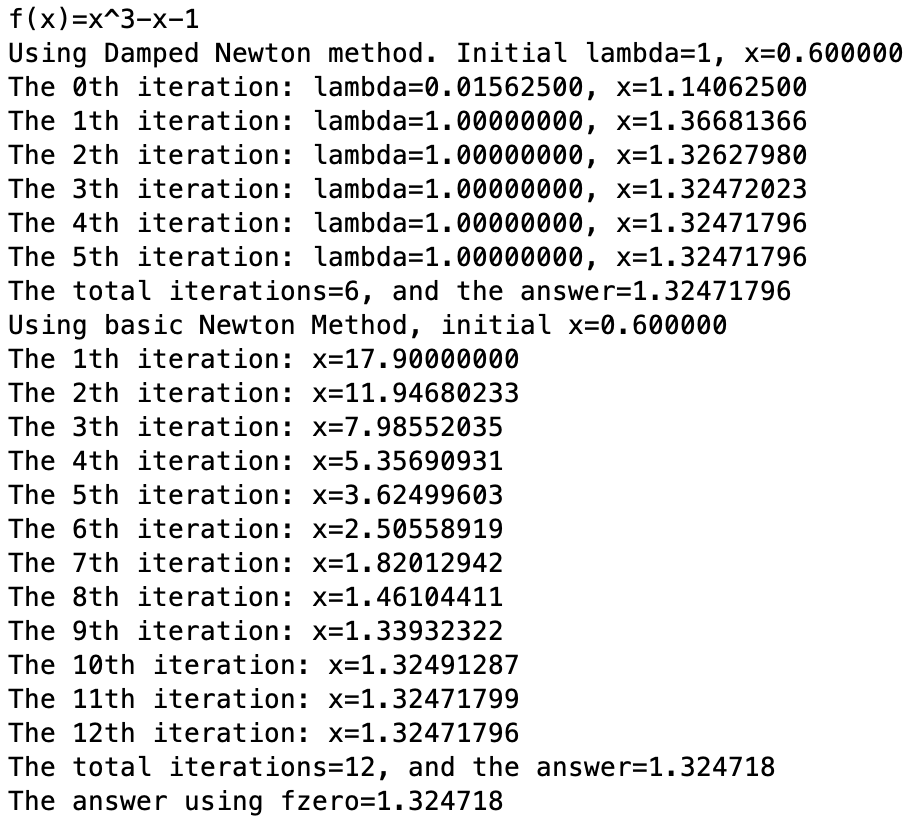
\includegraphics[scale=0.5]{photos/1.png}
\end{figure}
\begin{figure}[H]
	\centering
	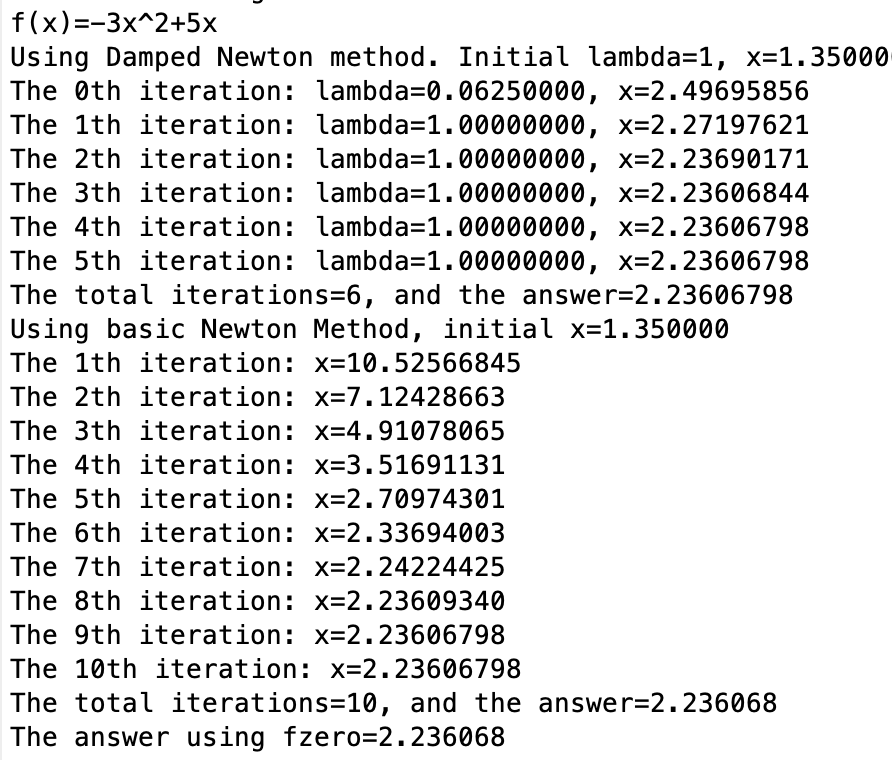
\includegraphics[scale=0.5]{photos/2.png}
\end{figure}

\subsection*{实验结论}
首先无论是基本的牛顿法还是阻尼牛顿法,求解结果都是十分准确的,至少在小数点后6位都和fzero得出的结果保持一致。改变阻尼因子的大小,发现其越小收敛速度越慢。

阻尼牛顿法引入的原因是当初始值$x_{0}$偏离解较远时,牛顿法可能会发散。因此增加单调性要求,使得$|f(x_{k+1})|<|f(x_{k})|$。当迭代解充分靠近准确解时,则不再要阻尼因子的调节。由于引入了阻尼因子,不仅避免了发散,也增加了收敛的速度。从实验结果中可以看出,使用阻尼牛顿法,两个方程都迭代了6次,而使用一般的牛顿法,则分别迭代了13次和11次,是两倍的关系。

另外,从结果中可以看出,两个方程都只有在第一次迭代时$\lambda$的值发生了变化,后面的迭代情况都比较理想。理论上,阻尼牛顿法也会出现情况很糟糕的时候。

\subsection*{实验心得}
这次实验是对书上的伪代码进行实现,不算太难。我主要了解了阻尼牛顿法的优点。建议可以增加一个该方法不好的例子。

\section{第二章第3题}
\subsection*{问题描述}
利用2.6.3节给出的fzerotx程序,在MATLAB中编程求第一类的零阶贝塞尔函数$J''(x)$的零点,$J''(x)$在MATLAB中通过命令besselj(0,x)得到。试求$J''(x)$的前10个正的零点,并绘出函数曲线和零点的位置。

\subsection*{解题思路}
根据fzerotx的定义,需要传入的参数有$J_0(x)$以及每个零点的所在区间。根据$J_(0)(x)$的性质,第i个零点所在区间为$[(i-1)\pi, i\pi]$。再调用fzerotx就能够得到想要的图像。

\subsection*{实验结果}
代码如下:
\lstinputlisting[language=Matlab, title=solve\_besselj.m]{../3/solve_besselj.m}
得到的十个零点为:
\begin{figure}[H]
	\centering
	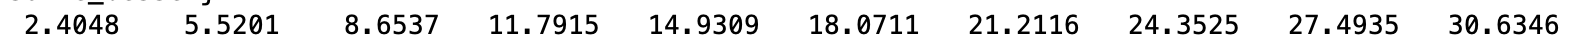
\includegraphics[scale=0.5]{photos/zeros.png}
\end{figure}
以及它们在图上的位置:
\begin{figure}[H]
	\centering
	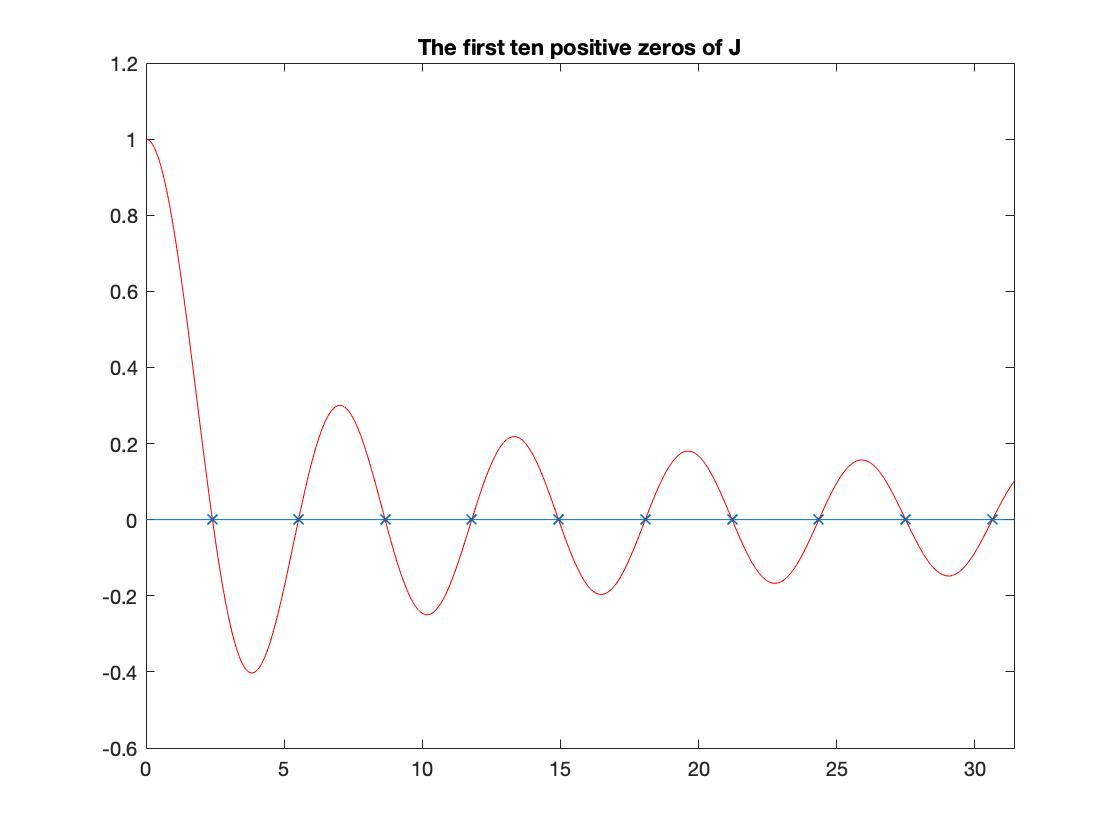
\includegraphics[scale=0.4]{photos/j0_zero.jpg}
\end{figure}

\subsection*{实验结论}
这次实验主要是调用fzerotx函数,本身并不困难。但是zeroin算法的理解需要花费一定功夫,而且从源码来看,其实现也相对比较复杂。最终求得的零点应当与理论十分契合,曲线相当优美。

\end{document}
